\subsection{Thermal Camera System}\label{thermal_system}

\subsubsection{Fundamentals of Thermal Imaging}\label{thermal_fundamental}

Thermal imaging is a passive, non-contact sensing technique that captures the \gls{IR} radiation naturally emitted by objects with temperatures above absolute zero\footnote{\label{thermography}\url{https://en.wikipedia.org/wiki/Thermography}}. Unlike visible-light cameras that rely on reflected light, thermal cameras measure emitted radiation and generate spatial maps of surface temperature.

The emission of thermal radiation follows the principles of blackbody radiation, where the intensity of emitted energy increases with surface temperature. Thermal cameras detect this radiation using infrared-sensitive sensors and convert the resulting signal into digital thermograms. These thermograms visualize temperature distributions: warmer objects emit more \gls{IR} radiation and appear brighter, while cooler objects emit less and appear darker\textsuperscript{\ref{thermography}}. The recorded thermal pattern depends not only on surface temperature, but also on material-specific thermal properties such as emissivity, conductivity, heat capacity, and density, which all determine how objects absorb and release heat over time.

In landmine detection, buried mines disrupt the natural thermal behavior of the soil. Due to differences in material composition, landmines and the surrounding soil exhibit distinct thermal inertia—their resistance to temperature change. As a result, the presence of a landmine creates a subtle but detectable thermal anomaly on the soil surface. Techniques such as Differential Apparent Thermal Inertia (DATI) can enhance these patterns by capturing the dynamic response of the soil and buried object to temperature changes over time~\cite{nikulin2018detection}.



\subsubsection{Thermal Camera Performance Parameters}\label{thermal_parameter}

The performance of a thermal imaging system depends not only on the physics of infrared radiation but also on the specific characteristics of the camera itself. Key parameters include the spectral band, thermal sensitivity, pixel resolution, \gls{FOV}, \gls{IFOV}, and \gls{GSD}. These factors collectively determine the system’s ability to detect small temperature differences, resolve fine spatial features from altitude, and identify landmines from the surrounding terrain.


\paragraph{Spectral Band}

The infrared spectrum is typically divided into five regions: Near-Infrared (NIR, 0.7--1.4~\textmu m)\glsused{NIR}, Short-Wave Infrared (SWIR, 1.4–3~\textmu m)\glsused{SWIR}, Mid-Wave Infrared (MWIR, 3–8~\textmu m)\glsused{MWIR}, Long-Wave Infrared (\gls{LWIR}, 8–14~\textmu m), and Far-Infrared (FIR, 15–1000~\textmu m)\glsused{FIR}. Among these, \gls{MWIR} and \gls{LWIR} are collectively referred to as the thermal infrared bands and are commonly used for passive thermal imaging due to their ability to capture emitted heat rather than reflected light\footnote{\label{LWIR}\url{https://www.shalomeo.com/LWIR-MWIR-Thermal-Imaging-Camera-shalomeo.html}}.

\gls{MWIR} and \gls{LWIR} provide temperature-based imaging that is robust under varied environmental conditions. Unlike \gls{SWIR}, which relies on reflected radiation, \gls{MWIR} and \gls{LWIR} sense emitted thermal energy, making them effective in low-light or obscured environments and well suited for buried landmine detection. According to Planck’s law, as an object’s temperature increases, its emitted radiation intensifies and shifts to shorter wavelengths. For objects near ambient temperature (300~K), peak emission occurs in the \gls{LWIR} range (8–12~\textmu m), making it the most appropriate band for detecting landmines both on the surface ad in the soil. In contrast, \gls{MWIR} is more effective for hotter objects (1000~K)\textsuperscript{\ref{LWIR}}. This relationship is illustrated in Figure~\ref{fig:wien_law}.

Atmospheric transmission also plays a role in band selection. Thermal imaging is most effective in atmospheric windows—wavelength regions with minimal absorption by water vapor and other gases. While \gls{MWIR} can perform slightly better in humid conditions, \gls{LWIR} benefits from a broader and more stable atmospheric window, making it ideal for terrestrial imaging in standard environments\textsuperscript{\ref{LWIR}} (see Figure~\ref{fig:atmos_window}).

\begin{figure}[h!]
    \centering
    \begin{subfigure}[b]{0.48\linewidth}
        \centering
        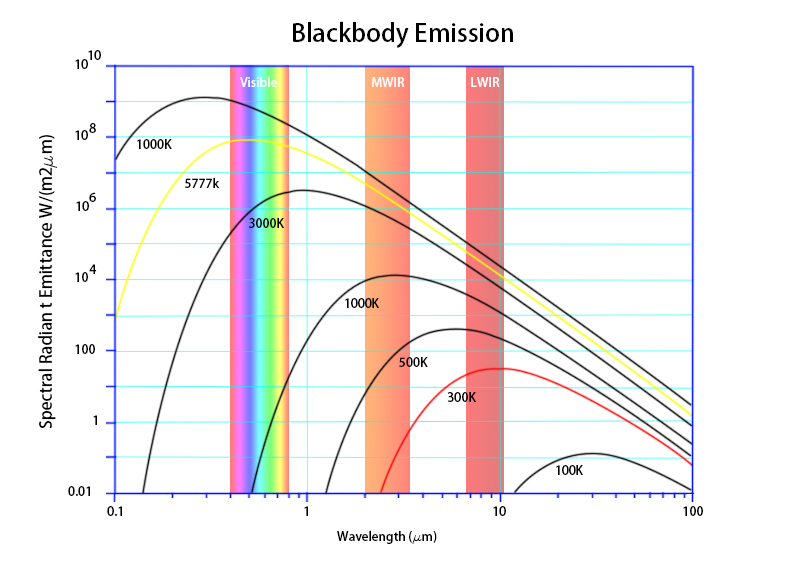
\includegraphics[height=3.5cm]{figs/Huirui/wien_law_plot.png}
        \caption{Planck spectral emission curve for different temperatures\textsuperscript{\ref{LWIR}}.}
        \label{fig:wien_law}
    \end{subfigure}
    \hfill
    \begin{subfigure}[b]{0.48\linewidth}
        \centering
        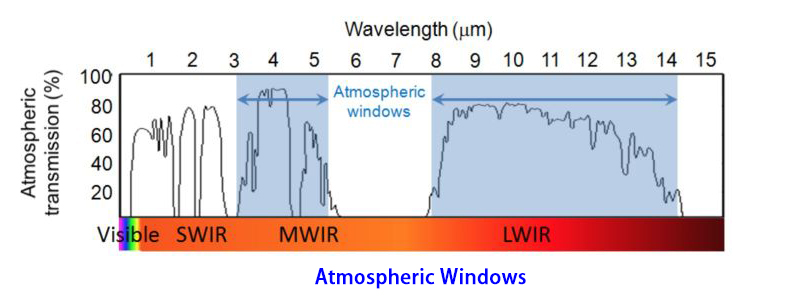
\includegraphics[height=3.5cm]{figs/Huirui/atmospheric_window_plot.png}
        \caption{Atmospheric transmission across infrared wavelengths\textsuperscript{\ref{LWIR}}.}
        \label{fig:atmos_window}
    \end{subfigure}
    \caption{Infrared sensing fundamentals.}
\end{figure}


Specific sensor design varies by spectral band as well. \gls{MWIR} cameras typically rely on cooled photodetectors made from semiconductor materials and require cryogenic cooling to reduce sensor noise. These systems provide high image quality but take much space, require lots of power, and is expensive. In contrast, \gls{LWIR} cameras usually employ uncooled microbolometer arrays, which detect temperature-induced changes in resistance, current, or voltage. While these sensors offer lower resolution and are more sensitive to self-heating effects, they are compact, lightweight, and energy-efficient\textsuperscript{\ref{thermography}}.

Given the need to detect subtle temperature differences under ambient conditions and the payload and power limitations of \gls{UAV} platforms, this project selects \textbf{\gls{LWIR}} as the preferred spectral band.


\paragraph{Thermal Sensitivity}

Also defined as \textbf{Noise Equivalent Temperature Difference} (NETD)\glsused{NETD}, thermal sensitivity is the smallest temperature difference that a thermal camera can detect, corresponding to a \gls{SNR} of 1. For example, a camera with a \gls{NETD} of 100~mK (0.1~\textdegree C) can theoretically distinguish a 25.1~\textdegree C object from a 25.0~\textdegree C background\footnote{\url{https://sierraolympia.com/what-is-netd-and-why-does-it-matter/}}. In practice, \gls{NETD} determines the sensitivity of the sensor to small thermal contrasts, which is critical for detecting the subtle temperature anomalies associated with landmines.

To estimate a realistic \gls{NETD} requirement, we refer to a laboratory study in which researchers used an infrared lamp to heat sand containing buried landmines, then monitored thermal signatures during passive cooling, which is an analog to solar heating in field conditions~\cite{lamorski2002thermal}. Table~\ref{tab:netd_table} summarizes the observed temperature differences at various burial depths and moisture levels from this research.


\begin{table}[H]
    \centering
    \footnotesize
    \renewcommand{\arraystretch}{1}
    \setlength{\tabcolsep}{6pt}
    \caption[Maximum temperature differences across moisture levels and depths]{Maximum temperature differences measured by thermocouples and infrared imaging under different moisture levels and burial depths~\cite{lamorski2002thermal}.}
    \label{tab:netd_table}
    \begin{tabular}{llccc}
        \toprule
        \textbf{Moisture Content} & \textbf{Measurement Type} & \textbf{2 cm Depth} & \textbf{3 cm Depth} & \textbf{4 cm Depth} \\
        \midrule
        \multirow{2}{*}{Dry sand} 
            & Thermocouple & 1.3 °C & 0.5 °C & 1.5 °C \\
            & IR Image     & 1.5 °C & 1.0 °C & -- \\
        \midrule
        \multirow{2}{*}{2.5\% water} 
            & Thermocouple & --     & 4.0 °C & 1.2 °C \\
            & IR Image     & 3.0 °C & 3.5 °C & 2.0 °C \\
        \midrule
        \multirow{2}{*}{5\% water} 
            & Thermocouple & 2.4 °C & 1.4 °C & 2.0 °C \\
            & IR Image     & 3.0 °C & 3.0 °C & 3.0 °C \\
        \midrule
        \multirow{2}{*}{10\% water} 
            & Thermocouple & 3.8 °C & 1.4 °C & 1.1 °C \\
            & IR Image     & 4.0 °C & 1.8 °C & 2.5 °C \\
        \bottomrule
    \end{tabular}
\end{table}


Although the experiment used a controlled heat source which is stronger than natural sunlight, it provides an upper bound on expected thermal contrast. In real-world outdoor settings, thermal differences are likely to be smaller due to deeper burial depth, slower heating, variable soil properties, and changing environmental conditions.

Accounting for these factors and the minimum temperature difference recorded from Table~\ref{tab:netd_table} (1.1~\textdegree C), and simulation results in~\ref{Results and Validation}, a conservative estimate for detectable temperature anomalies in practice is 0.5–1.0~\textdegree C. To resolve such differences reliably, a thermal camera with \textbf{\gls{NETD} ≤ 500~mK} is decided.


\paragraph{Pixel Resolution}

Pixel resolution refers to the number of individual sensing elements in a thermal camera’s detector array and determines the level of spatial detail of the system. It is typically expressed as width × height on the plane facing the camera, with common resolutions including 160×120 (low), 320×240 (medium), and 640×480 (high). Higher resolutions allow finer thermal detail and improved discrimination of small or partially obscured targets, which is essential for detecting landmines. However, increased resolution also raises sensor cost, power consumption, and weight\textsuperscript{\ref{thermography}}.

Since this project involves thermal scanning from relatively high altitudes, high resolution is necessary to preserve image clarity. At the same time, constraints on \gls{UAV} payload and system cost limit the use of ultra-high-resolution (1280×1024) cameras. This project selects a \textbf{640×480 resolution} as an effective compromise between performance and hardware feasibility.


\paragraph{FOV and IFOV}

The \gls{FOV} of a thermal camera defines the total angular extent within which the sensor can detect radiation. For drone-based applications where the camera is mounted in a nadir (downward-facing) orientation, the \gls{FOV} spans two angular directions—commonly referred to as the horizontal and vertical \gls{FOV}. In this aerial context, both directions lie in the horizontal plane relative to the ground: the horizontal \gls{FOV} determines the ground width of the captured area, while the vertical FOV corresponds to the ground length.

The \gls{IFOV}, by contrast, refers to the angular extent covered by a single pixel and directly determines the spatial resolution of the image. A smaller \gls{IFOV} means each pixel covers a smaller area on the ground, allowing for finer spatial detail.

Figure~\ref{fig:fov_ifov} illustrates the two-dimensional geometry of \gls{FOV} and \gls{IFOV}. In this simplified case, the thermal sensor is assumed to be square-shaped, with equal pixel resolution and physical dimensions along both axes. This implies symmetric angular \gls{FOV} and \gls{IFOV}, which simplifies calculations. In real-world cameras, however, differences may arise due to sensor shape or lens characteristics.

\begin{figure}[H]
    \centering
    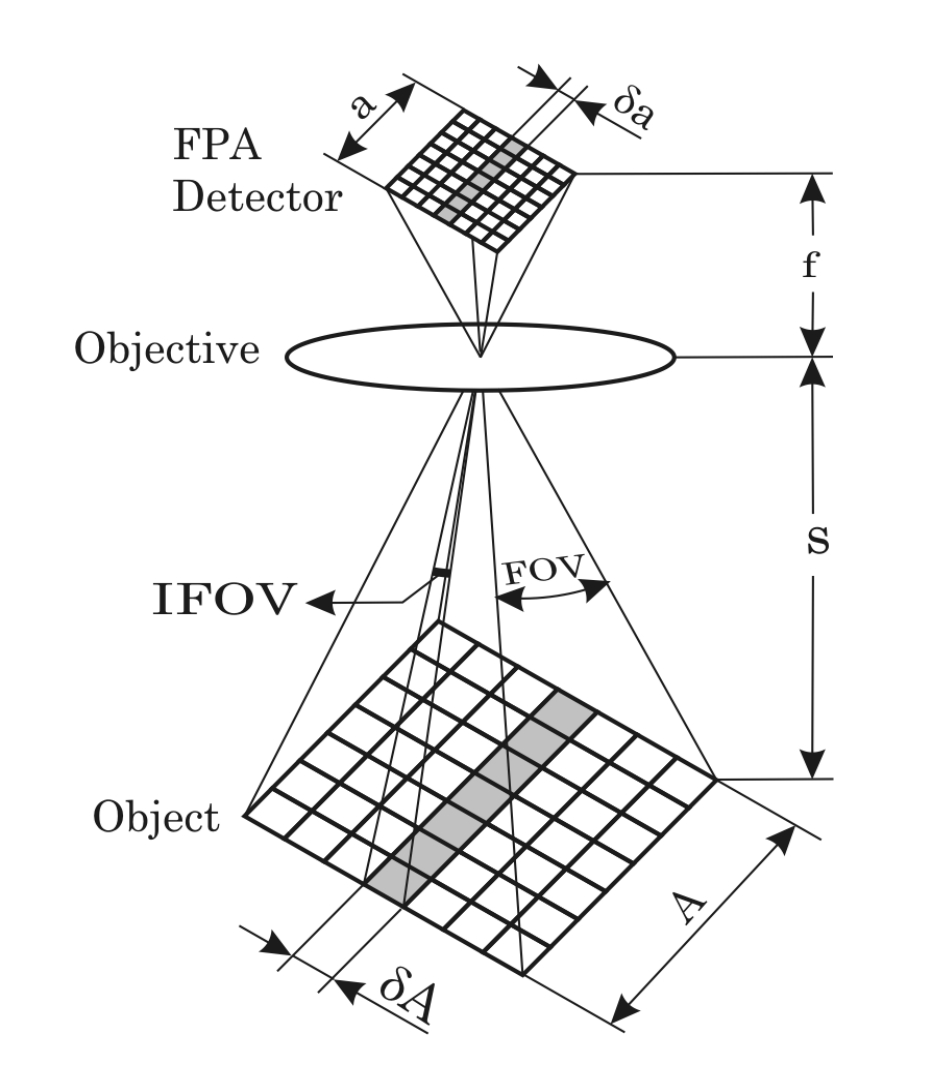
\includegraphics[width=0.3\textwidth]{figs/Huirui/fov_ifov_2d_diagram.png}
    \caption[Optical system FOV and IFOV]{FOV and IFOV for optical system~\cite{pencheva2006design}.}
    \label{fig:fov_ifov}
\end{figure}

Based on Figure~\ref{fig:fov_ifov}, the angular \gls{FOV} and \gls{IFOV} can be calculated as follows:

\begin{equation}
    FOV = 2 \cdot \tan^{-1} \left( \frac{a}{2f} \right) = 2 \cdot \tan^{-1} \left( \frac{A}{2S} \right)
    \label{eq:fov}
\end{equation}
\vspace{-1em}
\begin{equation}
    IFOV = 2 \cdot \tan^{-1} \left( \frac{\delta a}{2f} \right) = 2 \cdot \tan^{-1} \left( \frac{\delta A}{2S} \right)
\end{equation}

where \( f \) is the focal length of the lens, \( S \) is the height of sensor, \( a \) is the sensor width, \( \delta a \) is the pixel pitch, \( \delta A \) is the physical length represented between pixels, and \( A \) is total width of the ground area captured in the image.

For a fixed flying height and sensor resolution, a wider \gls{FOV} allows the drone to scan a larger area per frame, improving survey efficiency. However, it also increases the \gls{IFOV}, reducing the spatial detail of each pixel. Conversely, a narrower \gls{FOV} enhances resolution but limits coverage per frame. This trade-off is critical in drone-based landmine detection and must be evaluated collectively with the selection of flight altitude for this project in the section later.


\paragraph{Ground Sample Distance}

\gls{GSD} is the physical ground distance between each pixel in an image (represented as \( \delta A \) in Figure~\ref{fig:fov_ifov}). For example, in an image with a 1~m \gls{GSD}, adjacent pixels image locations are 1~m apart on the ground\footnote{\url{https://en.wikipedia.org/wiki/Ground_sample_distance}}. \gls{GSD} is determined by the drone’s altitude, the camera’s field of view, and the pixel resolution of the sensor.

Since \gls{APL}s typically have diameters ranging from 6 to 15~cm, as shown in Landmine section before, and we aim to achieve a resolution where at least 5–6 pixels span the width of a landmine, this leads to a target \gls{GSD} of approximately \textbf{1.4~cm/pixel}. This requirement directly informs our selection of flight altitude and \gls{FOV}, which will be discussed in the flight configuration section later.


\subsubsection{Thermal Camera Selection}\label{thermal_selection}

Based on the theoretical principles and performance criteria established in the previous sections, the thermal camera used in our drone system must satisfy several key constraints. First, it must operate in the \gls{LWIR} spectral range to align with peak thermal emissions from terrestrial objects at ambient temperature. Then, it should achieve a \gls{NETD} of no more than 500~mK to reliably detect subtle contrasts between landmines and surrounding soil. Moreover, a pixel resolution of at least 640×480 is required to capture sufficient spatial detail during high-altitude scanning. Additionally, the lens focal length and field of view must enable a \gls{GSD} of approximately 1.4~cm/pixel at flight altitudes between 5–10 meters. Finally, the camera’s weight and cost must be as low as possible.

Because a thermal camera’s resolution performance depends heavily on imaging geometry, we adopt a top-down approach: we first identify a suitable camera model, then derive the flight parameters (particularly altitude) needed to meet our spatial resolution (\gls{GSD}) target. This ensures that the selected hardware can realistically support the mission’s imaging requirements. The altitude calculation and coverage analysis are presented in the next section.

Due to time constraints and the complexity of hardware design, this project does not consider a customized thermal camera solution. Instead, we aim to identify a \gls{COTS} thermal camera based on sensors used in past research on drone-based thermal landmine detection across various environments and platforms~\cite{baur2020applying,nikulin2018detection,krause2018diurnal,TENORIOTAMAYO2024105567,FORERORAMIREZ2022104307,rs15040967,dena2020image,Fardoulis2020PROOFHS,butt2024uav,AgrawalChung2024ComparingSL,Popov2022MethodFM,TENORIOTAMAYO2023109443}. From these papers, we compiled a shortlist of \gls{LWIR} thermal cameras and summarized their key specifications, including pixel resolution, \gls{NETD}, \gls{FOV}, weight, and price, in Table~\ref{tab:camera_specs}.

Four models meet the minimum resolution requirement of 640×512 pixels: FLIR Vue Pro, FLIR Duo Pro R, FLIR Tau 2, and DJI Zenmuse XT. All fall within the estimated 4kg payload capacity of standard multi-rotor drones and offer excellent thermal sensitivity, with \gls{NETD} values below 50mK.


\renewcommand{\arraystretch}{0.9}
\setlength{\tabcolsep}{5pt}

\begin{table}[H]
    \centering
    \caption[Comparison of LWIR thermal camera models]{Comparison of LWIR thermal camera models used in previous studies.}
    \label{tab:camera_specs}
    \scriptsize
    \begin{tabular}{|c|c|c|c|c|c|}
    \hline
    \textbf{Thermal Camera} & \textbf{Pixel Resolution} & \textbf{\gls{NETD} (mK)} & \textbf{Lens \& \gls{FOV} (H × V)} & \textbf{Weight (g)} & \textbf{Price} \\
    \hline

    \textbf{FLIR Vue Pro\tablefootnote{\url{https://flir.netx.net/file/asset/10907/original/attachment}}} 
    & 640 × 512 & < 50 & 
    \begin{tabular}[c]{@{}c@{}}9 mm: 69° × 56° \\ 13 mm: 45° × 37° \\ 19 mm: 32° × 26° \end{tabular} 
    & 92–113.4 & 3895 (USD)\tablefootnote{\url{https://groupgets.com/products/flir-vue-pro}} \\
    \hline

    \multirow{2}{*}{\textbf{FLIR Duo Pro R\tablefootnote{\url{https://flir.netx.net/file/asset/8136/original/attachment}}}} 
    & 640 × 512 & < 50 & 
    \begin{tabular}[c]{@{}c@{}}13 mm: 45° × 37° \\ 19 mm: 32° × 26° \\ 25 mm: 25° × 20° \end{tabular} 
    & 325–375 & 6599 (USD)\tablefootnote{\url{https://www.tequipment.net/FLIR/DUO-PRO-R-640-19mm-9Hz/UAVs-and-Drones/}} \\
    \cline{2-6}
    & 336 × 256 & < 50 & 
    \begin{tabular}[c]{@{}c@{}}9 mm: 35° × 27° \\ 13 mm: 25° × 19° \\ 19 mm: 17° × 13° \end{tabular} 
    & 325 & 4499 (USD)\tablefootnote{\url{https://dronedoctorusa.com/products/flir-duo-pro-r-336-30hz-19mm-open-box}} \\
    \hline

    \textbf{FLIR One Pro\tablefootnote{\url{https://flir.netx.net/file/asset/14770/original/attachment}}} 
    & 160 × 120 & 70 & 50° × 43° & 36.5 & 349 (GBP)\tablefootnote{\url{https://www.flir.co.uk/products/flir-one-pro/?model=435-0006-03&vertical=condition+monitoring&segment=solutions}} \\
    \hline

    \textbf{FLIR One Edge Pro\tablefootnote{\url{https://flir.netx.net/file/asset/5631/original/attachment}}} 
    & 160 × 120 & 70 & 54° × 42° & 153 & 435 (GBP)\tablefootnote{\url{https://www.flir.co.uk/products/flir-one-edge-pro/}} \\
    \hline

    \textbf{FLIR Tau 2\tablefootnote{\url{https://www.unmannedsystemstechnology.com/wp-content/uploads/2012/04/FLIR-Tau2-Brochure.pdf}}} 
    & 640 × 512 & < 30 & 
    \begin{tabular}[c]{@{}c@{}}7.5 mm: 90° × 69° \\ 9 mm: 69° × 56° \\ 13 mm: 45° × 37° \\ 19 mm: 32° × 26° \end{tabular} 
    & 72 & 6813 (USD)\tablefootnote{\url{https://www.thermalvideo.com/46640001x.htm}} \\
    \hline

    \multirow{2}{*}{\textbf{DJI Zenmuse XT\tablefootnote{\url{https://www.dji.com/uk/zenmuse-xt/specs}}}} 
    & 640 × 512 & < 50 & 
    \begin{tabular}[c]{@{}c@{}}7.5 mm: 90° × 68° \\ 9 mm: 69° × 56° \\ 13 mm: 45° × 37° \\ 19 mm: 32° × 26° \end{tabular} 
    & 270 & 9900 (USD)\tablefootnote{\url{https://www.thedroneproshop.com/blogs/product-info/dji-zenmuse-xt-specifications}} \\
    \cline{2-6}
    & 336 × 256 & < 50 & 
    \begin{tabular}[c]{@{}c@{}}6.8 mm: 49.1° × 37.4° \\ 9 mm: 35° × 27° \\ 13 mm: 25° × 19° \\ 19 mm: 17° × 13° \end{tabular} 
    & 270 & 7999 (USD)\tablefootnote{\url{https://www.bhphotovideo.com/c/product/1318086-REG/dji_cp_zm_000337_zenmuse_xt_336x256_6_8mm.html}} \\
    \hline

    \end{tabular}
\end{table}


Among them, the FLIR Tau 2 provides the highest sensitivity (<30~mK) and is also the lightest (72~g), followed by the FLIR Vue Pro (92–113.4~g), DJI Zenmuse XT (270~g), and FLIR Duo Pro R (325–375~g). In terms of cost, the FLIR Vue Pro is the most affordable (3895~\gls{USD}), while the DJI Zenmuse XT is the most expensive (9900~\gls{USD}).

Although the DJI Zenmuse XT offers good performance, it is designed specifically for DJI drones and requires proprietary mounts, power connectors, and software protocols. Integration it with a custom \gls{UAV} would require hardware adaptation or even reverse engineering, which is not feasible within the time constraints of this project.

This leaves three practical options: FLIR Vue Pro, FLIR Duo Pro R, and FLIR Tau 2. All support standard PWM or serial interfaces and allow real-time video output via USB or analog ports. FLIR Duo Pro R is heavier and more costly than the Vue Pro, with no major performance advantage. FLIR Tau 2 offers slightly better sensitivity and weight, but is nearly twice as expensive.

Considering all these trade-offs, we select the \textbf{FLIR Vue Pro} as the thermal imaging solution for our system.



\subsubsection{Thermal System Flight Configuration}\label{thermal_flight}

With the FLIR Vue Pro camera selected, the next step is to determine appropriate flight parameters, including the operating altitude and \gls{FOV} (decided by lens focal length). It supports multiple focal lengths (9~mm, 13~mm, and 19~mm), each producing a different \gls{FOV}. Shorter focal lengths yield wider \gls{FOV}s, allowing larger ground coverage per image but at the expense of lower spatial resolution. In contrast, longer focal lengths provide narrower \gls{FOV}s, increasing resolution but reducing coverage area.

As established earlier, the target \gls{GSD} is approximately 1.4~cm/pixel. Given the fixed pixel resolution of 640×~512, and varying \gls{FOV}s across different lenses, we use geometric relationships to calculate the corresponding flight altitude for each lens option with the same coverage area.

Referring to Figure~\ref{fig:fov_ifov}, the \gls{GSD} \( \delta A \) is related to flight altitude \( S \) and camera resolution \( N \) via the following expression derived from Equation~\ref{eq:fov}:

\begin{equation}
\delta A = \frac{2 \cdot (S \cdot \tan(\frac{FOV}{2}))}{N}
\end{equation}

Rearranging, the required flight altitude to achieve a target \( \delta A \)  is:

\begin{equation}
S = \frac{\delta A \cdot N}{2 \cdot \tan(\frac{FOV}{2})}
\end{equation}

Using these equations, we evaluate each focal length option while holding \( \delta A \)  constant at 1.4cm/pixel. The resulting \( S \) are summarized in Table~\ref{tab:fov_results}.

\begin{table}[H]
\small
\centering
\caption[Flight height vs. focal length at 1.4~cm/pixel GSD]{Estimated flight height for different focal lengths (at GSD = 1.4~cm/pixel)}
\label{tab:fov_results}
\begin{tabular}{|c|c|c|}
\hline
\textbf{Focal Length (mm)} & \textbf{FOV (H × V)} & \textbf{Height (m)} \\
\hline
9  & 69° × 56° & 6.52   \\
\hline
13 & 45° × 37° & 10.82  \\
\hline
19 & 32° × 26° & 15.62  \\
\hline
\end{tabular}
\end{table}

From Table~\ref{tab:fov_results}, the required flight height increases substantially with focal length (from 6.52~m at 9~mm to 15.62~m at 19~mm). Since thermal radiation intensity diminishes with distance due to geometric spreading and atmospheric attenuation, flying at lower altitudes maximizes signal strength and image contrast. Therefore, the \textbf{9~mm} lens with flight altitude around \textbf{6~m} is selected as the optimal configuration.